Механическая игрушка~--- это игрушка, которая автоматически повторяет
определенную последовательность движений. В Японии механические игрушки
популярны с древнейших времен.

Движения механической игрушки управляются \textbf{схемой}, которая состоит из
\textbf{устройств}. Устройства соединены трубами. У каждого устройства есть любое
количество (возможно, ноль) \textbf{входов} и один или два \textbf{выхода}. Каждая труба
соединяет выход некоторого устройства со входом того же самого или другого
устройства. К каждому входу подключена ровно одна труба, и к каждому выходу
подключена ровно одна труба.

Чтобы описать, как работает схема, рассмотрим \textbf{шарик}, который в каждый
момент находится в одном из устройств. Шарик перемещается между
устройствами. На каждом шаге шарик покидает устройство, в котором он
находится, через один из его выходов, перемещается по трубе и попадает в
устройство на конце этой трубы через соответствующий вход.

Есть три типа устройств: \textbf{источник}, \textbf{триггер} и \textbf{переключатель}. Есть ровно один
источник, $M$ триггеров и $S$ переключателей ( может быть равно нулю). Вам
необходимо выбрать значение $S$. У каждого устройства есть уникальный
серийный номер.

Источник~--- это устройство, в котором в начале находится шарик. У него ровно
один выход. Его серийный номер равен $0$.

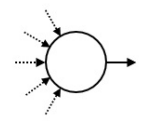
\includegraphics{1.png}


Триггер --- это устройство ровно с одним выходом. Серийные номера триггеров~---
целые числа от $1$ до $M$.

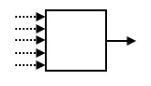
\includegraphics{2.png}

У каждого переключателя два выхода, которые обозначаются `X' и `Y'. Каждый
переключатель находится в одном из двух \texttt{состояний}: `X' или `Y'. После того, как
шарик попадает в переключатель, он покидает его через выход, равный текущему
состоянию переключателя. После этого переключатель меняет своё состояние на
противоположное. В начале каждый переключатель находится в состоянии `X'.
Серийные номера переключателей~--- целые числа от $-1$ до $-S$.

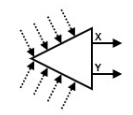
\includegraphics{3.png}

Задано количество триггеров $M$. Также задана последовательность $A$ длины $N$,
каждый элемент которой~--- серийный номер триггера. Серийный номер триггера
может встречаться в последовательности $A$ несколько раз (возможно, ноль). Вам
необходимо построить схему, которая удовлетворяет следующим требованиям:

\begin{itemize}
    \item Начав движение в источнике, шарик возвращается в источник после
нескольких перемещений.
    \item Когда шарик в первый раз после начала движения возвращается в источник,
каждый переключатель находится в состоянии `X'.
    \item Перед тем как шарик в первый раз после начала движения вернётся в
источник, он побывает в триггерах ровно $N$ раз. При этом он побывает в
триггерах с серийными номерами  $A_0,A_1,\ldots,A_{N-1}$ в этом порядке.
    \item Пусть $P$ равно общему количеству изменений состояний переключателей в
процессе перемещения шарика перед тем, как шарик впервые вернётся в
источник. Значение $P$ не должно превышать$20\,000\,000$.
\end{itemize}

При этом вы хотите использовать не слишком много переключателей.

\textbf{Детали реализации}

Вам необходимо реализовать следующую процедуру.

\begin{itemize}
    \item \texttt{create\_circuit(int M, int[] A)}
    \begin{itemize}
        \item $M$: количество триггеров.
        \item $A$: массив длины $N$, который задает серийные номера триггеров в том
порядке, в котором шарик должен в них побывать.
        \item Эта процедура будет вызвана ровно один раз.
        \item Обратите внимание, что число $N$~--- это длина массива $A$, которую можно
узнать методом, описанным в памятке о деталях реализации.
    \end{itemize}
\end{itemize}
Ваша программа должна вызвать следующую процедуру.
\begin{itemize}
\item \texttt{answer(int[] C, int[] X, int[] Y)}
\begin{itemize}
    \item $C$: массив длины $M+1$. Выход устройства с серийным номером $i$ ($0 \le i \le M$) iсоединён трубой с входом устройства с серийным номером $C[i]$.
    \item $X$, $Y$: массивы одинаковой длины. Длина $S$ каждого из этих массивов~---
количество переключателей. Для переключателя с серийным номером $-j$ ($1 \le j \le S$) его выход `X' соединён трубой с входом устройства с серийным
номером $X[j-1]$, а его выход `Y' соединён трубой с входом устройства с
серийным номером $Y[j-1]$.
    \item Каждый элемент массивов $C$, $X$ и $Y$ должен быть целым числом в диапазоне от $-S$
до $M$, включительно.
    \item $S$ должно быть не более $400\,000$.
    \item Процедура должна быть вызвана ровно один раз.
    \item Схема, описываемая массивами $C$, $X$ и $Y$, должна удовлетворять требованиям,
описанным в условии задачи.
\end{itemize}
\end{itemize}


Если одно из условий, перечисленных выше, не выполняется, ваша программа
получает вердикт \textbf{Wrong Answer}. Иначе ваша программа получает вердикт
\textbf{Accepted} и ваши баллы вычисляются по формуле в зависимости от значения $S$
(смотрите раздел <<Подзадачи>>).



